\documentclass[a4paper,11pt]{article}
\usepackage[colorlinks=true,linkcolor=blue,allcolors=red]{hyperref}
\usepackage{graphicx}

\renewcommand\thefootnote{\textcolor{red}{\arabic{footnote}}}
\renewcommand{\abstractname}{Definición}

\title{\LARGE \bf 
    Nonfunctional Requirements
}
\author{\\\\ Cristian Camilo Serna Betancur \\\\ Andres Grisales Gonzalez  
\\\\ John Fredy Mejia Serna}

\begin{document}
\maketitle
\tableofcontents
\begin{abstract}
    Un requisito no funcional o atributo de calidad es un requisito que sabe 
    bien y especifica criterios que pueden usarse para juzgar la operación de 
    un sistema en lugar de sus comportamientos específicos.\cite{DEFINITION}
\end{abstract}

\section{Performance}
El rendimiento define qué tan rápido un sistema de software o su pieza en 
particular responde a las acciones de ciertos usuarios bajo cierta carga de 
trabajo. En la mayoría de los casos, esta métrica explica cuánto debe esperar 
un usuario antes de que ocurra la operación destino.

\section{Wrapability}
Es la capacidad que tiene un sistema para ser \emph{envuelto} por otro sistema, 
logrando de este modo, adjuntar nuevos comportamientos y proporcionando 
funcionalidades adicionales manteniendo intacto el sistema principal. Dicho de 
otro modo, agregar funcionalidad a un sistema existente sin alterar su 
estructura actual.

\begin{figure}[!h]
    \centering
    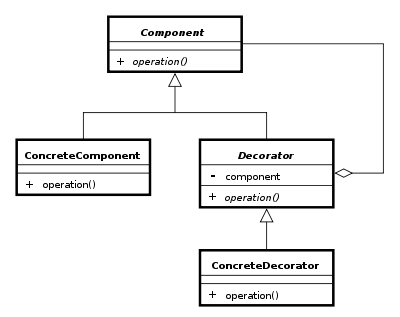
\includegraphics[scale=.7]{assets/decorator.png}
    \caption{Decorator Pattern}
\end{figure}

\section{Usability}
La \emph{usabilidad} es un requisito clásico no funcional\cite{USABILITY} que 
responde a una simple pregunta: ¿Qué tan difícil es usar el producto?

\subsection{Criterios de Usabilidad}
Pueden existir muchos tipos de criterios de usabilidad\footnote{Cabe destacar 
que cada persona podria tener sus propios criteros ya que no existe un concenso 
que lo especifique (como era de esperarce).}, a continuacion presentamos 
algunos de ellos:

\subsubsection{Capacidad de aprendizaje}
Que tan rápido es para los usuarios completar las acciones principales una vez 
que ven la interfaz.

\subsubsection{Memorabilidad}
¿Pueden los usuarios volver a la interfaz después de un tiempo y comenzar a 
trabajar de manera eficiente con ella de inmediato?

\section{Desacoplamiento}
Cuando hablamos de \emph{acoplamiento} nos referimos a la relación entre dos 
entidades en un sistema de software (generalmente clases).  Cuando una clase 
usa otra clase, o se comunica con ella, se dice que ``depende" de esa otra 
clase, por lo que estas clases están ``acopladas". Al menos uno de ellos 
``sabe" sobre el otro. La idea es que deberíamos tratar de mantener el 
acoplamiento entre clases en nuestros sistemas lo más ``flojo" posible: de ahí 
``acoplamiento suelto" o, a veces ``desacoplamiento". De esta forma, una de las 
tantas maneras para evitar este acoplamiento, es el uso de interfaces.

\section{Aciclicidad}
Con la \emph{aciclicidad} buscamos evitar dependencias cíclicas entre clases y 
entre paquetes, es una muy buena métrica para medir la mantenibilidad del 
software, cuando nos encontremos con dependencias cíclicas debemos sentarnos un 
rato y pensar como modificamos ya sea la ubicación de clases dentro paquetes de 
manera que podamos romper esa ciclicidad que es dañina.  

\subsection{Ejemplos}
\begin{figure}[!h]
    \centering
    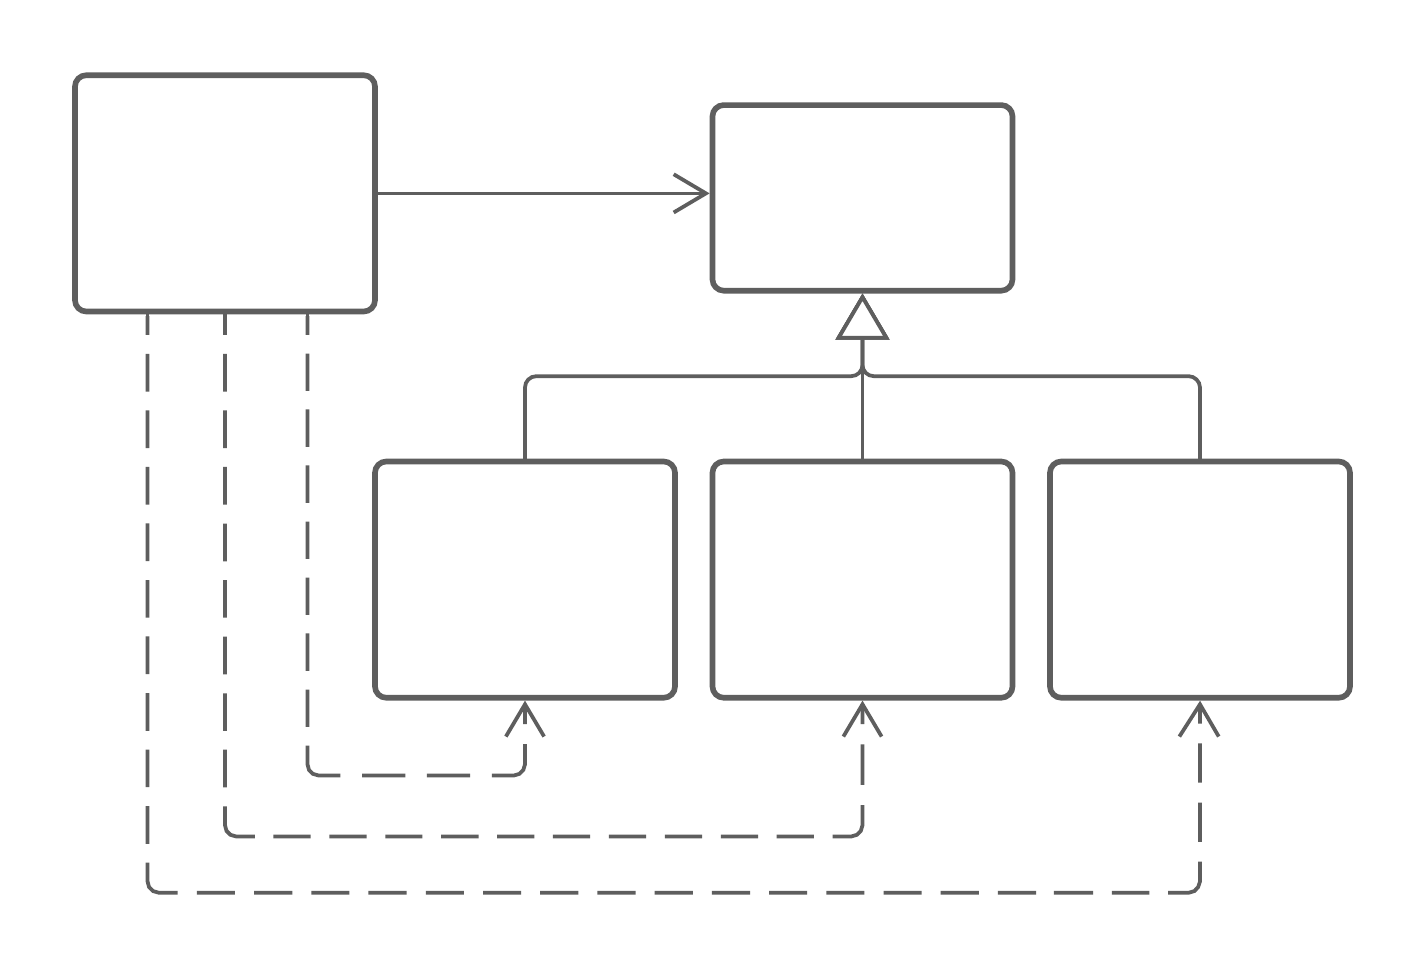
\includegraphics[scale=.7]{assets/ec1.png}
    \caption{Esto no está bien.}
\end{figure}

\begin{figure}[!h]
    \centering
    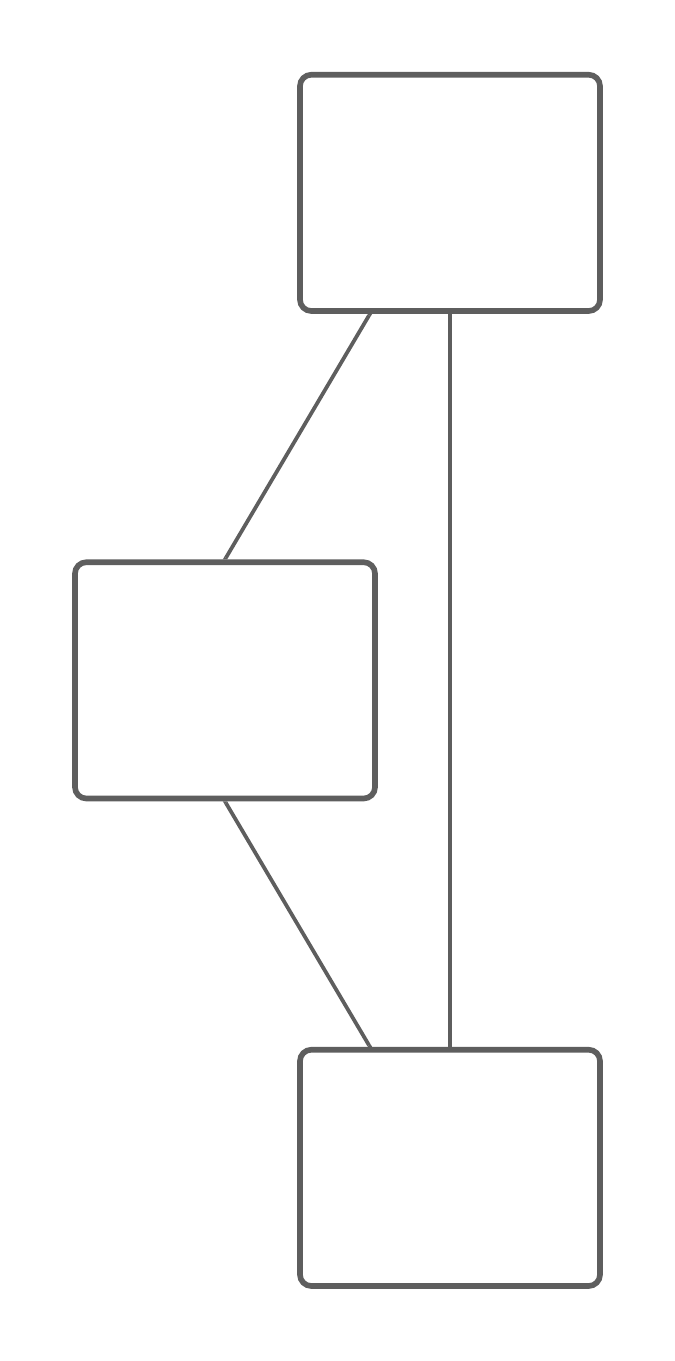
\includegraphics[scale=.7]{assets/ec2.png}
    \caption{Esto tampoco está bien.}
\end{figure}

\begin{figure}[!h]
    \centering
    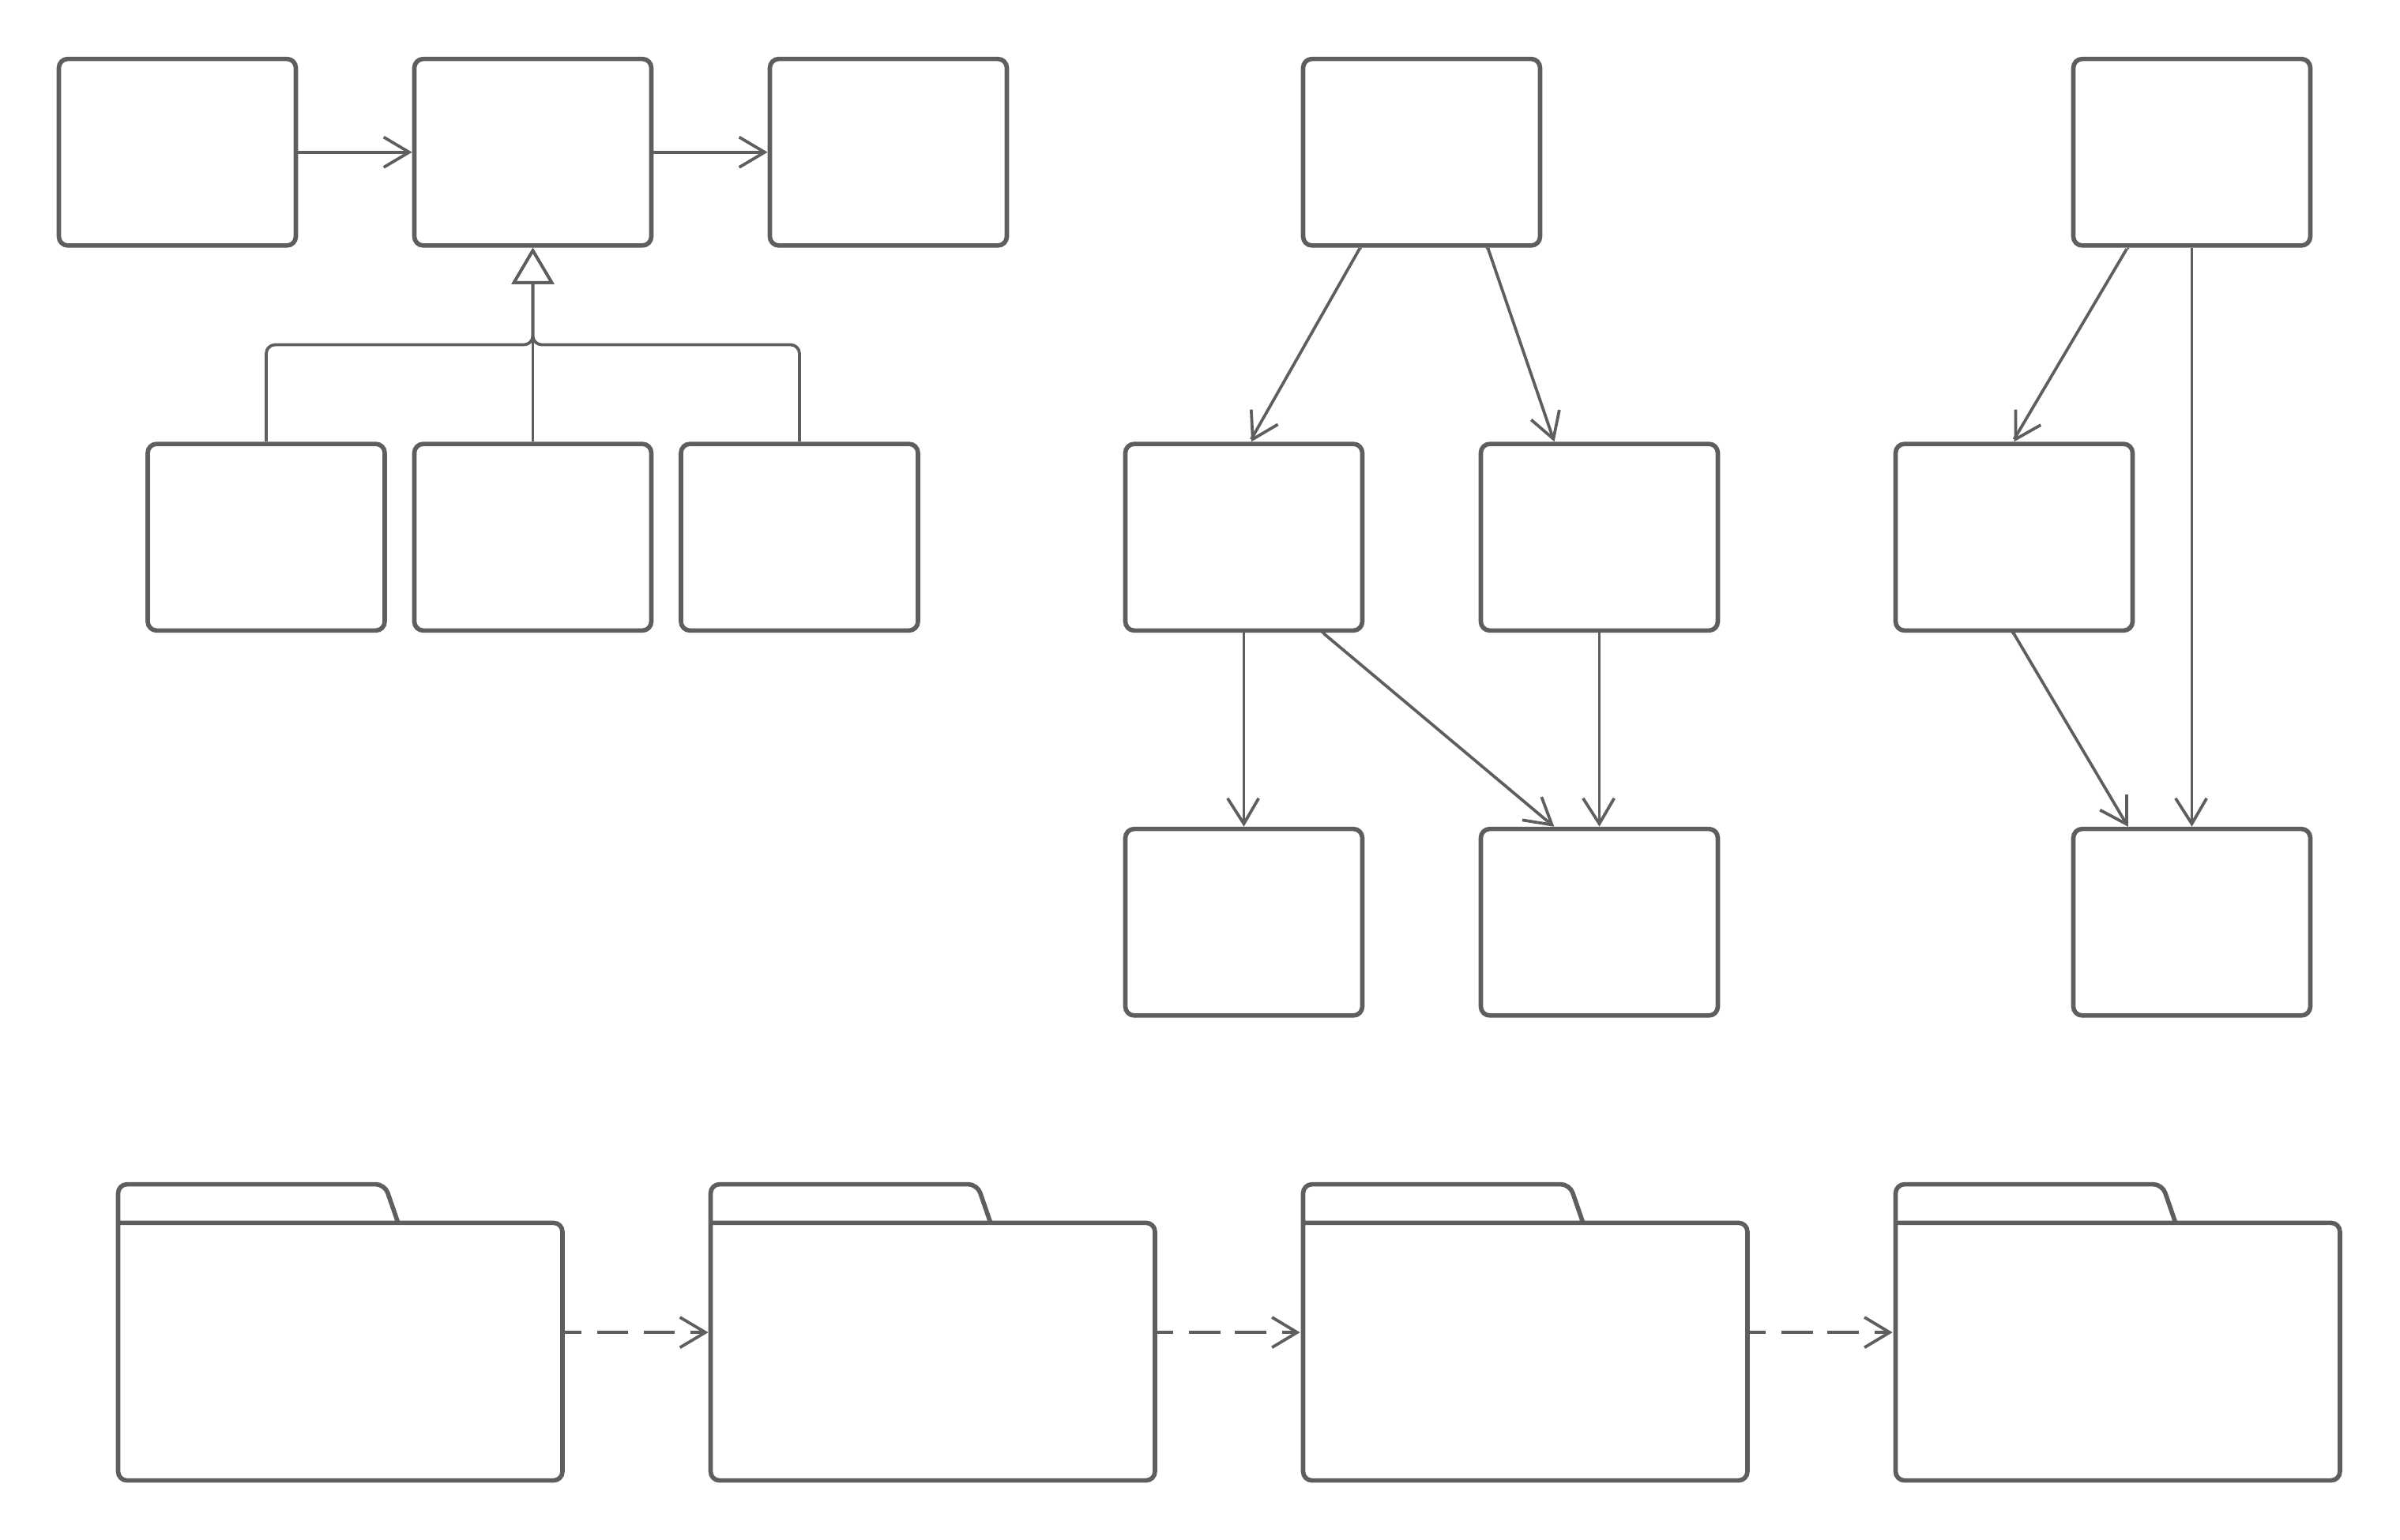
\includegraphics[scale=.5]{assets/gc1.png}
    \caption{Esto está bastante bien.}
\end{figure}

\section{Sustituibilidad}
Buscamos la capacidad de \emph{substitución} correcta de subtipos de una clase, 
la forma de tener una sustituibilidad adecuada es respetando correctamente el 
Principio de substitución de Liskov.

\bibliography{nonfunctional-requirement}{}
\bibliographystyle{plain}
\end{document}
